%%%%%%%%%%%%%%%%%%%%%%%%%%%%%%%%%%%%%%%%%%%%%%%%%%%%%%%
%
% AUTHOR: 李顺
%
% DESCRIBTION: 论文第一章部分
%
%
%%%%%%%%%%%%%%%%%%%%%%%%%%%%%%%%%%%%%%%%%%%%%%%%%%%%%%%

\chapter{绪论}
\label{chap:intro}
\section{选题的背景和意义}
无人机(UAV)技术在近年来得到了极其迅速的的发展。其中,尤其是固定翼无人机被广泛应用于现代战争之中。但是单架无人机往往限制较多,例如
:由于机载传感器尺寸、安装位置以及精度的限制,单架无人机往往不能快速全面的侦察某一广泛区域的战略目标;由于单架无人机隐蔽性以及机动性的限制,
单架无人机受到敌方打击而失效的概率大大增加。

而多架无人机进行编队控制从而进行协同作战可以使得无人机群体的战场存活率相较于单无人机系统更高。另外,通过图像拼接、协同滤波等技术
可以将编队侦查的无人机系统的信息融合为整个大环境的整体态势,因而
编队无人机对于战场的侦查效率也大大提高,对于单一传感器的精度的要求也相应降低。从而能
更好的完成领土保卫以及战场侦察任务。除此之外,无人机进行紧密编队还可
以实现长航程、长航时任务中无人机的空中加油等任务, 如图\ref{fig:c01-meaning}所示,从而进一步提高了无人机的作战能力以及适应复杂战场环境的能力。

固定翼无人机以紧密编队的方式飞行,如迁徙的鸟儿一样,可以减少整体的飞行阻力并且减少燃料消耗。整体编队产生的气动减阻效果将会
精心设计的、
具有良好的气动外形的飞行器相媲美。但是,按照相关文献显示,如果固定翼编队的控制精度无法达到要求精度的10\%,那么最优的减租效果
可能会被削减30\%。\cite{Zhang2017Aerodynamics}此外,固定翼编队避障也是热点问题之一:2019年,张佳龙等人对三架无人机的协同编队以及
其避障做了相关研究。\cite{Zzhangjialong2019Collision}

小型低成本固定翼无人机因其体积小巧、携带简单、部署容易以及成本低廉等优点,逐渐成为进行固定翼无人机编队实验的良好平台。\cite{Wangxiangke2019}通过现有的开源自动驾驶仪再结合机器人操作系统
配合商业级自动驾驶仪可以方便进行无人机编队的仿真以及实物试飞实验。
固定翼无人机编队飞行实现涉及队形规划、编队形成、队形保持与变换、协调通信甚至编队避障等领域。相较于四旋翼等空中机器人的编队,固定翼
因其动力学模型的复杂性,直接导致控制上的复杂性,进而使得固定翼自主编队的任务更加困难。另外因为控制硬件成本的低廉性,导致控制精度的下降,
使得编队控制将更加困难。本文旨在提出一种符合固定翼无人机动力学特性
的、基于当前较为成熟的开源无人机自动驾驶仪的固定翼紧密编队软件、硬件解决方案。
 \begin{figure}[H]
  \centering
  \subfigure[无人机编队加受油]{
  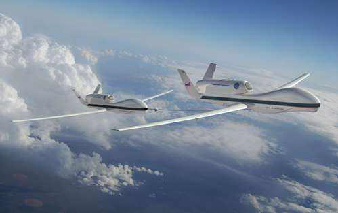
\includegraphics[width=0.45\textwidth, height=0.25\textwidth]{figures/c1/c01-meaning-1} 
}
  \subfigure[无人机编队巡航]{
  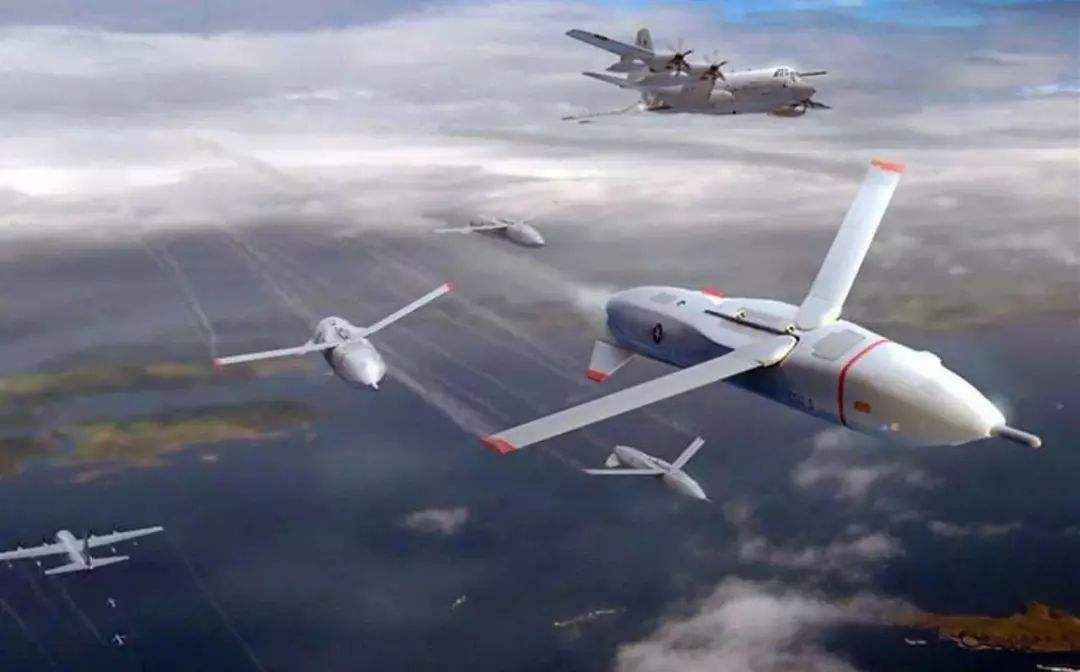
\includegraphics[width=0.45\textwidth, height=0.25\textwidth]{figures/c1/c01-meaning-2}
}
  \subfigure[无人机编队协同作战]{
  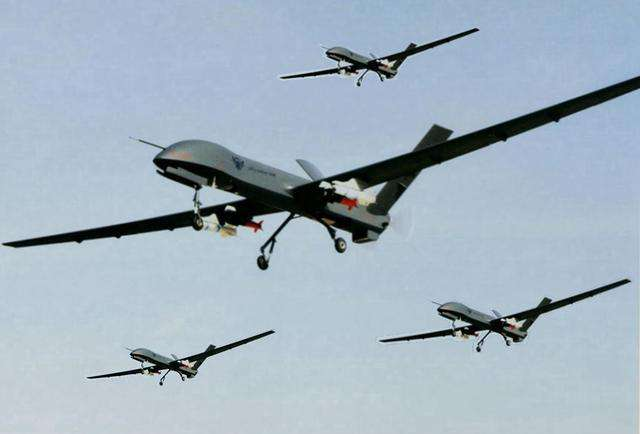
\includegraphics[width=0.45\textwidth, height=0.25\textwidth]{figures/c1/c01-meaning-3}
}
  \subfigure[无人机编队信息交互]{
  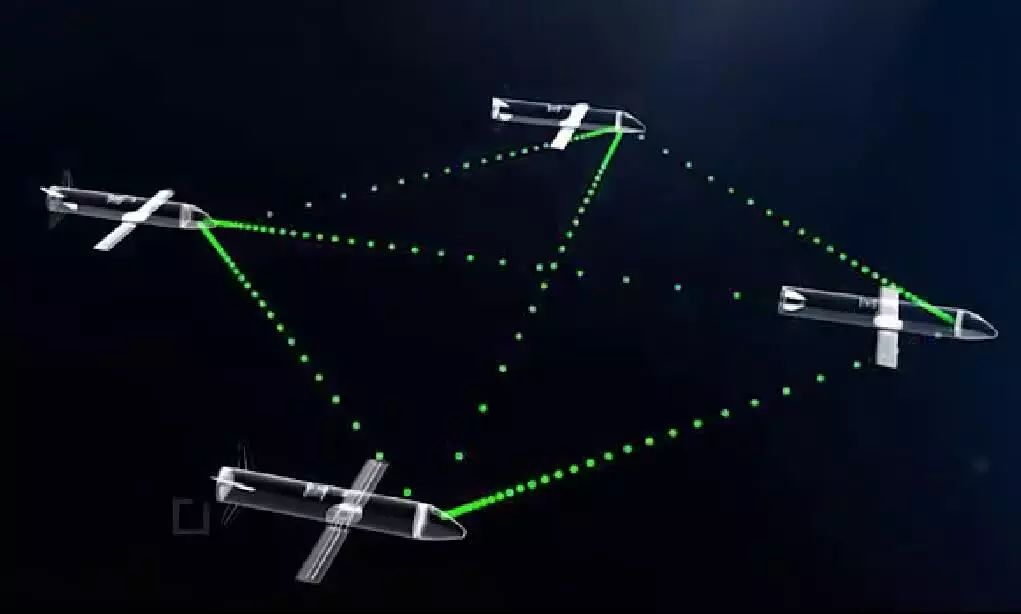
\includegraphics[width=0.45\textwidth, height=0.25\textwidth]{figures/c1/c01-meaning-4}
}
  \caption{无人机编队应用场景}
  \label{fig:c01-meaning}
  \end{figure}
\section{国内外研究现状及发展趋势}
\subsection{无人机自动驾驶仪发展}
自动驾驶仪是无人机自主飞行的核心控制单元,更是链接飞行任务以及无人机的软件、硬件桥梁。
成熟的无人机自驾仪应至少具备决策、航迹规划,状态感知和数据采集以及飞行控制等功能,从而实现无人机的自主决策、自主飞行,最后完成既定飞行任务。
任务的完成性。\cite{LiuLi2010}
现如今的开源无人机自动驾驶仪的结构多分为由姿态估计模块、任务与通信模块、导航模块、位置外环控制控制模块以及姿态内环控制模块等;其中,导航与
位置模块的典型控制器形式有传统或者改型后的数字式PID控制器、L1控制器\cite{Park_2004}与TECS控制器等\cite{Lambregts1983Vertical};导航模块根据当前位置以及飞行任务产生位置期望值,位置控制模块
由导航模块产生的期望位置产生
姿态角期望值,姿态控制模块由期望姿态角产生最终的伺服系统的控制量。图\ref{fig-c1-autopilot}展示了一款典型的固定翼无人机自动驾驶仪逻辑。
\begin{figure}[H]
    \centering
    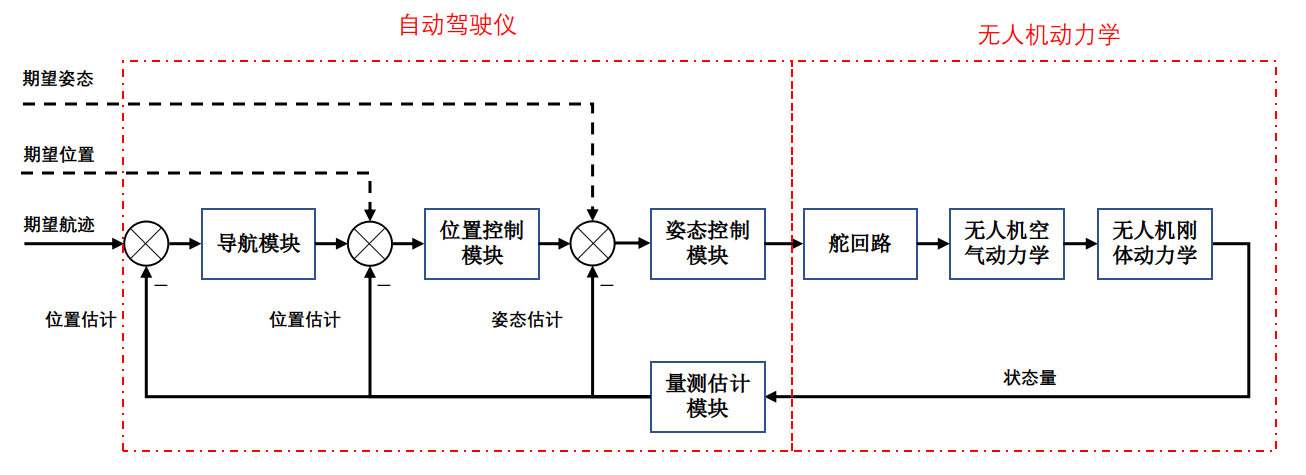
\includegraphics[width=0.85\textwidth]{figures/c1/autopilot_struct}
    \caption{典型无人机自动驾驶仪结构}\label{fig-c1-autopilot}
\end{figure}
\subsection{编队控制算法发展状况}
多无人机编队的最终目的是在空间之中形成固定的亦或是随时间变化的期望几何形状。
就目前国内外的研究成果而言,编队控制器可以按照是否涉及多无人机协同分为两类:不涉及协同控制理论的,多采用集中式的结构,编队结构中,选择现有无人机
或者生成虚拟位置点作为编队中无人机的参考点,控制的目标是每一架无人机获得期望的位置以及速度,最终消除位置以及速度等运动量上的误差,达到编队的
目的。此种方法思路明了直接,容易进行实际应用,对于通信链路的带宽以及可靠性的要求不高,适合低成本的无人机部署使用;其缺点也十分明显:编队网络中的
无人机之间缺少甚至不能进行充分的状态信息交互,如果关键节点的功能丧失,则有可能引起整体编队的发散。

涉及协同控理论的编队控制方法,通过无人机之间的信息交互,可以使得编队中的无人机获得与自己相邻无人机的信息,从而进行运动上的协调,各个无人机共同
调节消除编队误差;另外,分布式的网络相较于集中式网络有着可靠性上的巨大优势。缺点则以现在对通信要求提高以及实现成本之上。

另外,按照编队形成的方法上,现如今的编队方法有如下几种:
\begin{enumerate}
    \item 人工势场法\\
        此方法的本质也是一种基于距离的编队控制方法,类似于物理学中电场、磁场等概念,将无人机的运动看作是在一种人为假设的力场中运动,期望位置点将对
        无人机产生“引力”,若存在障碍物点,则改点对于无人机产生“斥力”。最终的控制量是无人机所受到的“合力”。在2014年,金远先等人利用改进的人工势场法
        对无人机编队控制器进行了设计,并做了相关的仿真验证。\cite{Jin2014}
    \item 基于行为的方法\\
        基于行为的控制方法定义了几种计算的“目标”,例如位置追踪、飞行避障以及队形保持等。将无人机编队过程中的
        不同“目标”的比重进行加权,得到最终的控制量,但是方法本身约束较少,产生的效果常常为松散编队,并且其稳定性难以在数学上给出明确的证明。
        2008年,Lazea等人考虑了地面机器人的绝对以及相对位置之后,利用基于行为的编队方式进行编队控制,并做了相关的仿真验证。
    \item 领从方法\\
        领从方法指在编队过程中,选择一架或几架无人机作为编队的领航无人机,其飞行航迹预先给定;编队中的其余无人机作为跟随无人机,获取领航无人机
        的相关状态信息,之后结合自身位置以及期望编队位置,得出编队控制的误差进而设计合理的控制器形式消除之,达到编队目的。此方法原理简单,应用较为广泛。
        早在2007年,西北工业大学的朱战霞、郑莉莉等人在从机机体坐标系之中设计了基于PI控制器的编队控制器,分别用于机体纵向以及机体侧向,并
        提出了编队的混合误差定义。\cite{ZhuZhanXia2007}
        2009年,Kim等人考虑无人机的动力学模型之后,设计出了一种非线性的双机编队控制器模型。\cite{Kim2009A} 2019年,Ben M.CHEN等人结合协同控制的相关理论
        ,针对无人直升机的编队做了相关设计以及实验。\cite{Ben2010Design}
        魏扬等人在2016年设计出一款基于PID控制器的输出控制量为期望加速度以及偏航角的编队控制器,并结合飞行器的二阶积分模型对控制器做了稳定性的数学证明。\cite{WeiYang2016}
    \item 虚拟结构法\\
        虚拟机构法假定编队的期望队形为空间中的刚体,每一架无人机通过追踪给定的虚拟结构上的特征点进而完成编队。此种方法避免了领从方法对于领航无人机的
        通信依赖,但是其对于通讯的要求仍然较高。另外由于其不能描述任意形状的空间几何体,如今的虚拟结构法只被用在多边形的编队上。
        虚拟结构法常通过虚拟领机方法将群体无人机协同起来。在1996年,KarHan等人在解决机器人编队的过程中提出了虚拟结构法的概念。\cite{Tan1996Virtual}
    \item 虚拟领机法\\
        虚拟领机法的主要思想是为编队中的每一架无人机都设计一个虚拟领机,但是其复杂性会随着编队无人机的增加而加大。2007年,Sun等人结合虚拟领机
        以及人工势场法为陆地无人车编队设计了一种鲁棒控制器。\cite{Sun2007}
        2018年,秦澍祺等人针对四旋翼无人机的编队问题,设计出了一种基于虚拟领机的分布式
        编队控制算法。\cite{Qin2018}哈尔滨工程大学的薛多锐在2019年为解决水下自制机器人的混杂编队问题
        提出了一种基于虚拟领航方法的编队控制方法。\cite{Xue2019}
\end{enumerate}
值得注意的一点是:无人机编队的控制方法并不是完全相互独立的,例如在上述的介绍的虚拟结构法之中,编队时的虚拟领机的计算需要使用协同控制相关理论生成期望的
虚拟领机的位置,而在编队的控制阶段(形成阶段),对每一架无人机而言,将使用类似于领从方法控制本无人机消除与虚拟领机的期望误差,因而单就编队形成阶段而
言,并不涉及协同控制理论。另外,上述方法之间也可以相互结合形成新的编队方法。例如:Pan W. W.等人在2017年将虚拟结构法与人工势场法进行结合,针对多无人水下
机器人的编队问题设计出了相应的控制算法。\cite{Pan2017A}2019年,吕永申将类似的思想应用到了多无人机集群编队控制之中。\cite{Lv2019}

最近几年新型的控制器逐渐被应用到编队控制器的设计之中:2011年,西北工业大学肖亚辉等人针对无人机的三维编队设计了一种具有良好鲁棒性的模糊PID控制器,进而控制无人机的三维编队。\cite{XiaoYaHui2011}
2018年,南京航空航天大学的许玥将自适应容错控制器引入到编队控制器的设计之中来。\cite{XuYue} 2019年,赵菁祥等人设计了编队控制的
滑膜控制器。2020年,北京理工大学的强佳久设计了参数优化自抗扰固定翼无人机编队控制器。\cite{MengXiuyun2020}近年来,还有的学者考虑到无人机编队问题中的时变问题,
并作出了先关的研究,例如:何吕龙等人利用图论的相关知识研究通信拓扑等相关问题\cite{Helvlong2020};类似的还有周绍磊\cite{Zhoushaolei2020}、张西勇\cite{Zhangxiyong2019}等人的研究;
董朝阳\cite{Dongzhaoyang2020}、季蕾\cite{Jilei2019}、徐振\cite{Xuzhen2019}等人则研究了编队结构中的时变问题。

现如今已经存在的大部分编队控制算法均为考虑飞机的质点运动学以及质点动力学条件下提
出的导航方法,最终产生的飞行器的控制量为无人机航迹坐标系下的加速度期望值以及无人机的航向角的期望角速度。例如:朱战霞、魏扬等人所设计的编队控制器
按照飞机的控制方式,需要将航迹坐标系下的
期望控制量转到机体系之下,但是飞机自动驾驶仪并不能接受加速度控制量,尤其是飞机机体$O_bx_b$轴方向,无人机推力、阻力以及重力沿机体方
向的推力并非是代数关系,不能直接由期望加速度得到期望推力;无人机姿态驾驶仪常使用协调转弯模型作为内环角度环的控制基础,不能直接响应
所给出的偏航角速度的期望值。2019年吉林大学的张天慧基于上述介绍的领从方法,利用地面站与自动驾驶仪系统设计固定翼编队控制器,\cite{Zhangtianhui2019}但是
其方法规划与运算由地面站完成,延时以及不确定性相较机载计算平台增加。总结而言即:
当前的大部分编队控制律不能很好的与自动驾驶仪内环相结合结合。
但是现如今的低成本无人机所使用的传感器硬件精度比较低,均为消费级别,如果不考虑传感器的精度问题而设计控制方案,很可能导致整体编队的控制精度下降。
另外由于低成
本无人机的惯性原件的精度问题导致无人机不能使用测量的加速度信息作为反馈,两种原因导致以加速度为最终控制量对于低成本无人机编队的方法控制精度不足。
\section{本文的内容安排}
本文中的编队控制器设计基于开源自动驾驶仪内环以及编队控制的领从方法,从无人机编队的距离、速度大小以及速度方向误差出发,设计符合现有无人机内环姿态驾驶仪输入的
编队控制器。
本文之后的部分将如下组织:第二章首先介绍编队控制设计的假设以及所用到的坐标系,最终建立建立无人机编队的动力学模型。之后介绍自动驾驶仪的控制逻辑:包括导航、位置控制以及姿态控制等模块的实现。第四章首先
完成对于编队误差的定义,将所定义的编队误差作为输入、无人机内环姿态驾驶仪期望姿态作为输出,设计编队控制器数学形式;第四章介绍
无人机编队整体控制逻辑、动力学仿真环境以及硬件选型 ;第五章控制器仿真以及实际飞行实验结果分析;最后为结论。
